\begin{figure}[htb]
\centering
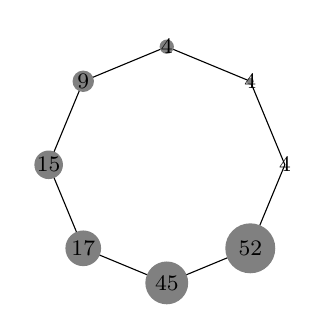
\begin{tikzpicture}
\def\cradius{1.5};
\def\cliqueradius{0.001};
%\draw[help lines,step=1] (0,-5) grid (10,5);
\edef\counter{0};
\def\sizes{{ 4, 4, 4, 9, 15, 17, 45, 52}};

\draw (0:\cradius)
\foreach \x in {0,45,...,315}{ -- (\x:\cradius) }-- cycle (90:\cradius) node[above] {};

\foreach \angle in {0,45,...,315}{
      \def\cliquer{ {\angle * 0.001} };
      
      \pgfmathsetmacro{\pg}{\sizes[\counter]}; % set the macro pg with the current value of counter
      \counter
      \fill[black, thick,fill=gray] (\angle:\cradius) circle (\angle * 0.001);
      \node[black] at (\angle:1.5) {{\footnotesize $\pg$}};
      \pgfmathparse{\counter + 1}; \xdef\counter{\pgfmathresult}; % increment counter and store the result again in counter
      }
\end{tikzpicture}
\label{fig:ring_of_clique_powerlaw}
\caption{Power-law ring of cliques, $\min_c=5$, $\max_c=75$, $n=150$, $\tau_c=1$}
\end{figure}